\clearpage\section{SafeDE Evaluation}

This section assesses SafeDE by different methods in the context of De-RISC MPSoC. To perform the evaluation process, we simulated the VHDL model of the MPSoC, including SafeDE IP. For that purpose, we used the simulator QuestaSim. We also synthesized the platform into a Xilinx Kintex UltraScale KCU105 evaluation kit and performed several tests. 

\subsection{Functional Validation}

This section assesses SafeDE by different methods in the context of De-RISC MPSoC. To perform the evaluation process, we simulated the VHDL model of the MPSoC, including SafeDE IP. For that purpose, we used the simulator QuestaSim. We also synthesized the platform into a Xilinx Kintex UltraScale KCU105 evaluation kit and performed several tests. 

Several strategies are applied to validate the correct SafeDE functionality:

\textbf{Testbench:} The first approach to validating SafeDE is using a VHDL testbench that simulates the system's behavior by generating SafeDE inputs and reacting to its outputs. For that purpose, a component simulating the behavior of the cores is developed. This component generates the inst\_cnt signals for both cores, randomly setting its bits to '1' as if the cores were committing instructions. If the stall signal of one core is set to '1', this prevents the \textit{inst\_count} signal bits of that core from being set to '1' as it would in a real core. 

In addition to this component,  procedures are defined at the testbench top to simulate APB read and write transactions. These procedures allow configuring the internal SafeDE registers during the simulation. As mentioned before, SafeDE has some statistic registers that can be read through the APB interface. During the testbench execution, the same statistics are computed at the top of the testbench so they can be compared with the results recovered from SafeDE. 

Therefore, the testbench execution starts configuring internal SafeDE registers. After that, the testbench runs for a configurable number of cycles simulating two cores executing instructions that hold when the stall signals rise. Finally, SafeDE is stopped and the statistics are retrieved. The testbench pass provided that the statistics read from SafeDE registers and the statistics computed at the top of the testbench coincide and the staggering keeps all the time between the limits ($Min\_TH_{stag} < \#intst_{head} - \#inst_{trail} < Max\_TH_{stag}$).

The testbench completion is the first step for SafeDE design validation and it also eases the development process since the testbench is automatically run each time a new Git push is performed, informing of potential errors each time the design is modified.



\textbf{RISC-V ISA tests:} RISC-V ISA tests \cite{ISAtests} are a group of tests designed by the University of California to test the correct functioning of the RISC-V ISA instructions. The ISA tests are written in a single assembly language file and contain a self-checking code to test the result. Each ISA test tests one operation from the RISC-V ISA forcing corner cases. 

To load the binaries into the platform, control the execution flow and debug the application, we used GRMON. GRMON is a general debug monitor for the LEON (SPARC V7/V8) processor, NOEL-V (RISC-V) and for SOC designs based on the GRLIB IP library developed by CAES Gaisler. 

We modified the RISC-V ISA tests assembly code to configure and activate SafeDE prior to the test execution. We also performed some modifications to perform the execution in two different cores. The linker script is modified to load two ISA tests in two different address segments. GRMON is employed to activate both cores and determine the correct entry point. Once the test has finished, the results are stored in one register file register in each core. Those registers are read using GRMON to test that each test successfully passed. 

This process is automated via Makefiles (for the compilation), Bash scripts and GRMON TCL scripts. Therefore, a simple Linux command compiles the binaries, uploads the binaries to the FPGA, controls the execution flow and checks the results for all of the selected RISC-V ISA tests. The correct completion of these tests proves that neither the internal modifications performed to the integer pipeline of the cores nor the SafeDE action produces any system malfunctioning.

\textbf{TACLe Benchmarks:} TACLe Benchmarks suite \cite{falk2016taclebench} is a set of self-contained and open-source benchmarks of varying types and sizes. They are specifically designed for the evaluation of critical real-time embedded systems. Since they are self-contained, they have their inputs hardcoded together with the source code, making them perfect for experimenting in a bare metal setup. Their execution times range from thousand of cycles to a few millions of cycles, making them, in many cases, easy to simulate and debug to understand unexpected results.

We ported some TACLe Benchmarks to RISC-V ISA and added some C functions from the bare metal drive to configure SafeDE and gather execution statistics. As with the RISC-V ISA tests, TACLe Benchmarks also have a self-checking function that compares the obtained results (or a signature summarizing the final result) and the expected results. TACLe Benchmarks are executed over the FPGA loaded with the De-RISC platform bitstream. Execution is controlled by GRMON. The compilation, loading and result checking processes are automated using different scripts. 

We checked for all the executed TACLe Benchmarks that the results with SafeDE forcing 20 instructions of staggering ($Min\_TH_{stag} = 20; Max\_TH_{stag} = 32750$) coincide with the expected results. Also, results from the statistic registers are gathered for every benchmark. We checked that in every execution, the number of executed instructions by both cores coincide and that the minimum staggering reached during the execution is never below that of the expected one ($staggering > Min\_TH_{stag} = 20$). Note that the maximum staggering threshold value is high enough to not interfere in the execution.

Since a 1-cycle latency exists between the moment the stall signal is asserted until the core pipeline stops making progress, the former staggering condition does not hold all the time during the execution of the benchmarks. Since cores are dual-issue, they can commit two instructions each cycle, being the worst scenario the one in which, with a previous 21 instructions staggering, the trail core commits two instructions while the head core commits none. When this happens, the staggering reaches 19 instructions, and trail core stall signal rises. Since that signal will take effect the next cycle, the trail core can commit another two instructions while the head cores commit none again, leaving the staggering at 17 instructions. The same happens for $Max\_TH_{stag}$. The real minimum staggering that is kept is dependent on the architecture, namely on the number of issues of the core and the number of cycles that elapses from the moment the stall signal is asserted until it stalls the pipeline. 

\bigskip



\subsection{Fault Injection}
We perform a simulation-based fault injection campaign to test the De-RISC platform CCFs detection capabilities when SafeDE is active. We added VHDL non-synthesizable logic to the pipelines of the NOEL-V cores. This logic randomly injects faults in different pipeline locations. Namely, faults are injected in:

\begin{itemize}
    \item \textbf{ALU:} Each core has two ALUs which have two 64-bit inputs (one per issue). The fault is injected in one bit of one of the inputs from one of the ALUs. The ALU, its input and the input bit are randomly selected. 
    \item \textbf{Late ALU:} Each core has two late ALUs that help to handle data dependencies efficiently. Each late ALU has two 64-bit inputs. The fault is injected in one bit of one of the inputs from one of the late ALUs. The late ALU, its input, and the input bit are randomly selected.
    \item \textbf{Memory:} In the pipeline memory stage, a fault is injected in a random bit of the data about to be written into the data L1 cache.
    \item \textbf{Write back:} The pipeline write back stage has two 64-bit write ports to write the data in the register file. One bit from the write ports is randomly selected to insert the fault.
\end{itemize}

Three different fault models are simulated during the fault injection campaign: stuck-at-0, stuck-at-1 and bit flip. The targeted bit for the fault injection is set to '0' for the stuck-at-0 model, to '1' for the stuck-at-1 model and to the logical opposite value for the bit flip. At first, simulated faults were of one cycle of duration. However, we found that most of the injected faults were masked. For that reason, a second fault injection campaign was performed, increasing the fault durations to 10 cycles. In the case of the bit flip model, the bit is flipped in the first cycle, and the value is kept during the nine subsequent cycles.

Simulation-based fault injection requires a lot of computation capacity and can take a long time to complete. To shorten the experimentation time, we chose a concrete TACLe Benchmark: FAC, one of the shortest TACLe Benchmarks. Before launching the experiments, our intuition was that only CCFs that cannot be detected using a lockstepped execution regardless of its implementation (hardware/software tight/light) would go unnoticed. Those insights proved to be right for the selected benchmark FAC.

The code of the benchmarks is executed in both cores simultaneously. SafeDE is configured to impose a minimum staggering threshold of 20 instructions and a maximum staggering threshold of 32750 instructions (value pre-defined when the user does not set the maximum staggering). Although the staggering will never reach the maximum threshold due to its big value. The fault could be injected at any cycle provided that both CritSec registers are activated. Hence, the fault is randomly injected at any cycle between the moment the trail core starts its critical region until the head core finishes it. The fault location is randomly selected among the ones mentioned above. The fault is injected in the same location and simultaneously in both cores emulating a CCF.

To analyze the simulation results, we take advantage of the TACLe Benchmarks routine to check if the execution results coincide with the expected results. With this, we know if both execution outputs were correct or not. In addition, a VHDL procedure to dump the memory contents into a file is designed. After each simulation, memory dumps of both cores are compared to each other and the golden run memory dump. During the execution, the core could try to perform a store operation outside the memory limits. In a real execution, this could produce a segmentation fault if the application is running over an operating system. The core could also modify internal registers of a peripheral unintendedly. For that reason, a VHDL procedure was designed to monitor the AHB interface and detect any transaction outside the memory limits.

\begin{itemize}
    \item \textbf{Timeout:} Simulation time exceeds by three the fault-free simulation time of the benchmark.
    \item \textbf{Crash:} The simulation process is terminated abnormally.
    \item \textbf{Software detected:} The software comparison detected a mismatch between both core execution results. This category includes latent memory errors that differ between cores. Hence, they are not immediately detected by the comparison mechanism, but if they eventually manifest, they would do as different execution outputs.
    \item \textbf{Identical memory SDC:} Both executions produce the same memory corruptions (SDC) and could potentially cause the same incorrect execution results, making it impossible for the comparison mechanism to detect the failures. It is detected using the memory dumps.
    \item \textbf{DUE:} One of the cores wrote outside its memory limits, causing a non-recoverable error. The AHB monitoring detects it.
    \item \textbf{Masked:} The fault is masked when the outputs and memory contents are equal to the ones of the golden run.
    \item \textbf{Undetected error:} The execution results were different from the golden run, but they coincide between both cores. In this case, software comparison does not detect the error and SafeDE fails to protect the system against the CCF.
\end{itemize}


Table \ref{fault_injection_results} summarizes the results of the fault injection campaign. 4,000 simulations were performed for each fault model and duration. A total of 24,000 simulations were carried out. As shown, most of the injected faults are masked. As expected, the likelihood of a fault being masked decreases when the duration of the fault increases. Some faults led to a timeout or a crash, making the error easily detectable. Other faults produced different erroneous outputs in both cores and were detected by software comparison. Some of the simulations produced errors in memory, but in none of the cases, the errors were equal across both cores (identical SDC is always 0 for all the experiments). None of the fault-injection experiments led to a DUE. However, some injections classified in other categories (timeout, crash or software detected) wrote outside the memory limits.


 \begin{table}[h]
    \caption{Fault injection results classified by fault model.}
    \label{fault_injection_results}
    \centering
    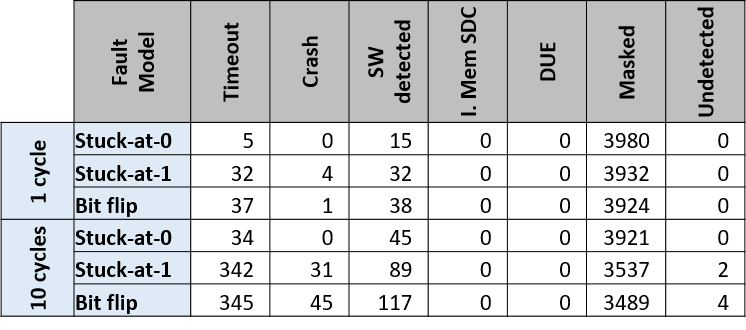
\includegraphics[width=1\columnwidth]{img/faultinjection2.png}
\end{table}
   

From all the simulations performed, the injected fault produced an error that the software comparison mechanism could not detect only in six. In all cases, the faults were injected in the write back stage. These errors led the system to a failure despite employing SafeDE to force a staggered execution. For that reason, we found it interesting to analyze those simulations in detail.


The benchmark FAC calculates the factorials from 0 to 12. Each result is accumulated in global variable. Finally, the value of this variable that contains the addition of all the factorials is compared to the expected result. FAC performs the factorial operation employing recursion. Figure \ref{fig:fac_assembly} shows the assembly code obtained after compiling the C code. We could distinguish three different sections: initialization, an outer loop that accumulates the factorial results and an inner loop that compute the factorials using recursion. 

In this particular case, the fault model is a bit flip that lasts 10 cycles. The bit selected to inject the fault is the least significant bit of the second write port of the register file, which flips to 1 and introduces an erroneous value in the write port. The fault is injected while the program is computing the factorial of 8. 

%%Rewrite it
However, those values are read through a bypass in the inner loop instead of from the register file, so no impact is observed in the inner loop. In the last iteration of the inner loop, the result of the factorial is stored in register a4 (line 8) with an erroneous value (due to the duration of the fault). Later, the register a4 is read as an operand for addw instruction in line 17, which accumulates all the calculated factorials. Therefore, this error is propagated to the output. Particularly, the erroneous result contains one bit flip in the least significant bit with respect to the correct result.

In the trail core, the fault is injected while the core is executing the outer loop. The fault affects several instructions, but all the errors except one are masked because they are either overwritten or not read since they are forwarded like in the head core. The error not masked is produced in line 17 when the result of the addition is written back to the a6 register, which stores the accumulation of the factorials. Again, the final value contains one bit flip with respect to the correct output in the least significant bit. Therefore, even though the fault affects both cores differently, in the end, it produces the same bit flip in the accumulated register (a6), which stores the output value.

Thus, the software is not capable of detecting the error, not because of a malfunctioning of SafeDE, but because of the semantics of the benchmark FAC. In fact, even if we used tight lockstepping, external core activity would be identical for both cores and no error would be detected. We content that, despite we could produce this apparent CCF in our fault injection campaign, such effect would be very unlikely to occur in practice since both cores have different states when the fault occurs, and this should lead to heterogeneous electric impact, hence causing heterogeneous errors (e.g., affecting only one core, or affecting different bits or locations of both cores).
%%%%%%%%%%%%

\begin{figure}[h]
    \centering
    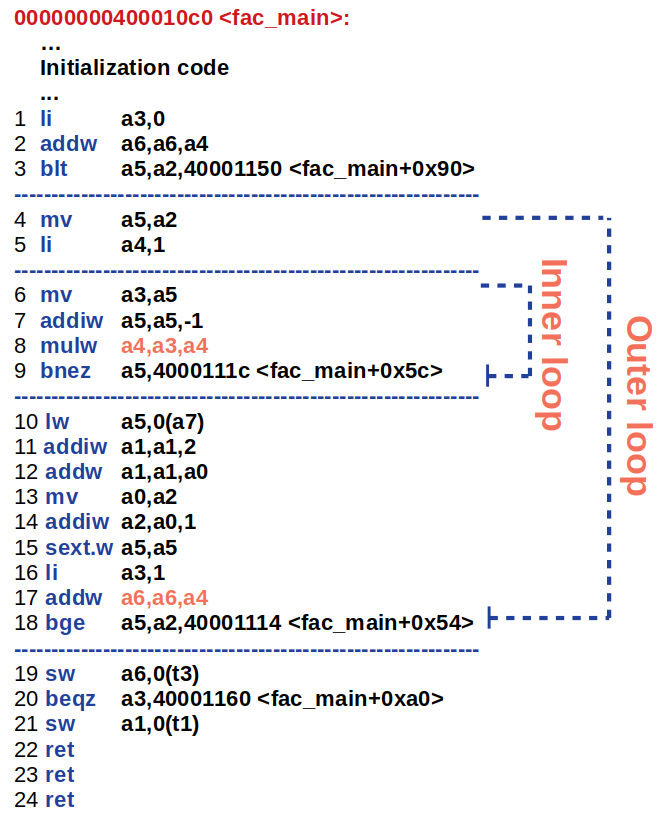
\includegraphics[scale=0.4]{img/fac_assembly.png}
    \caption{Excerpt of the assembly code of the benchmark FAC.} 
    \label{fig:fac_assembly}
\end{figure}

\bigskip



\subsection{Time Overhead}

To determine how much SafeDE afects the performance we have run the TACLe Benchmarks in three different scenarios:

\begin{enumerate}
    \item Isolation: Only one core executes the benchamrk while the other remains idle.
    \item Redundancy without diversity: Both cores execute the same benchmark without SafeDE enforcing any staggering. 
    \item Diverse Redundancy: Both cores run the same benchmark and SafeDE is active enforcing a staggering of 20 instructions ($Min\_TH_{stag}$ = 20)
\end{enumerate}

As stated before, it is convenient to set a staggering big enough to ensure that pipelines of both cores do not contain the same instruction in any of the pipeline stages at any point of the execution. Taking into account that NOEL-V cores are dual-issue with a 7-stages pipeline (pipelines can execute in parallel 14 instructions), 20 instructions of staggering (17 in practice) will suffice to avoid the two pipelines executing any common instruction. 

To generate two redundant processes, the same binary is loaded twice in different memory segments (one for each core). Each benchmark is executed 1,000 times to discard small variations across different executions due to random processes like the effect of the DRAM refresh in the memory latency. Although, the variation observed in the execution time between several executions of the same benchmarks has shown to be very low, in the order of a few tens of cycles.

Figure \ref{fig:tacle_results} shows the results. In the Figure, the execution time for redundancy without diversity and for diverse redundancy are normalized w.r.t the execution time in isolation. Results show that SafeDE computational overhead is really low. Namely, when SafeDE enforce diverse redundancy performance degrades by 0.3\% on average (up to 0.6\% for BITONIC) w.r.t executions in isolation, and 0.003\% (up to 0.6\% for IIR) on average w.r.t redundant executions without diversity. 

\begin{figure}[h]
    \centering
    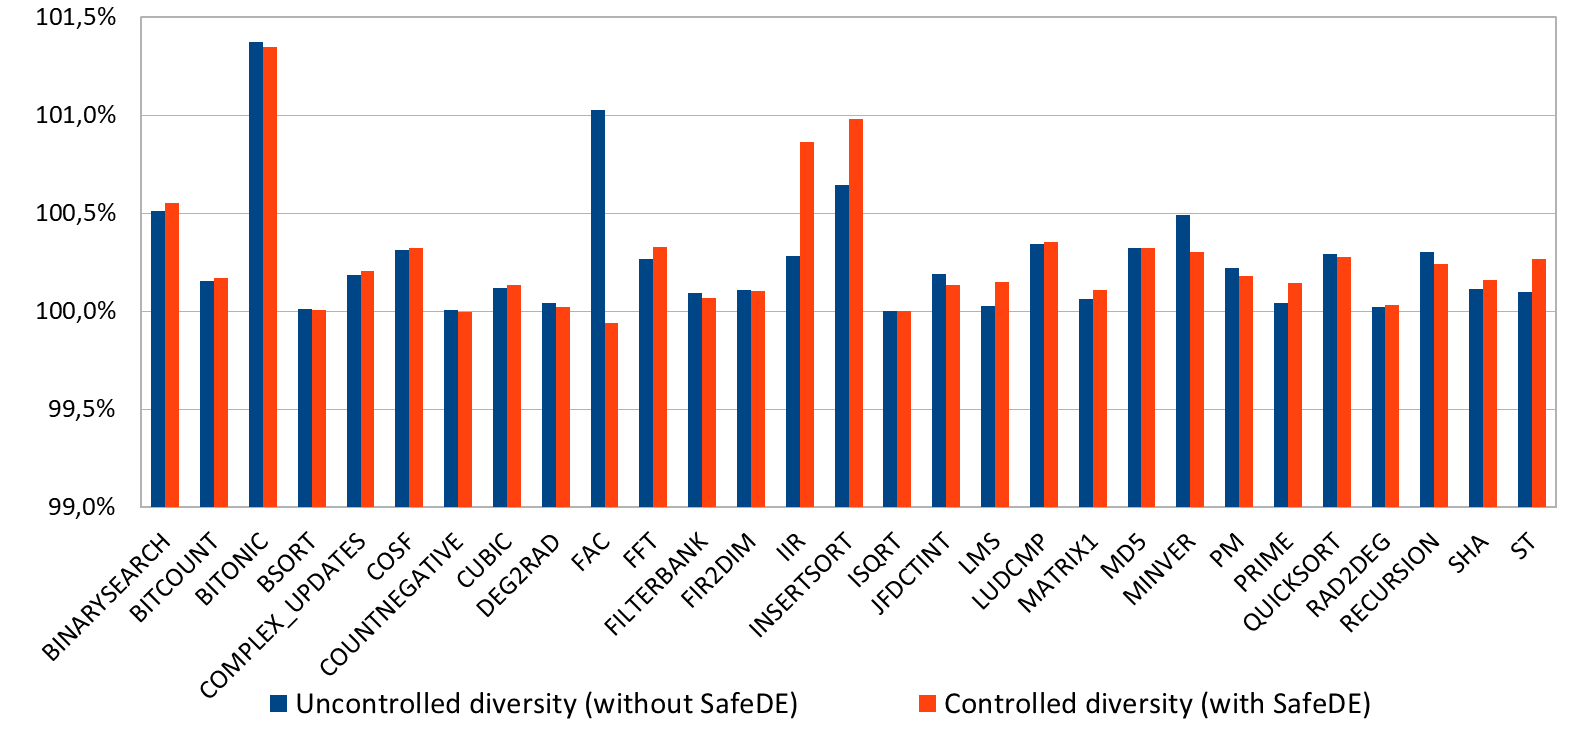
\includegraphics[scale=0.6]{img/tacle_results.png}
    \caption{Execution time of different TACLeBench benchmakrs normalized w.r.t. their execution time in isolation. Each benchmark is executed 1,000 times.}
    \label{fig:tacle_results}
\end{figure}


Results for Fac benchmark execution show that the execution time with controlled diversity is shorter than the execution time in isolation. To explain this anomalous result, we performed two simulations to compare the isolation run against the diverse redundancy execution. After a close examination, we found that the branch predictor was behaving differently, causing minor variations in both executions. These variations have a more significant impact in relative terms in smaller benchmarks like Fac, which executes only around 700 instructions. 

Summing up, execution time increase with diverse redundancy is negligible. SafeDE allows configuring small staggering thresholds, as we did in our evaluation (20 instructions), which are way below than those allowed by the software-only solution \cite{alcaide2020software}, positioning SafeDE as a much more efficient solution for light-weight lockstepped execution. 


\bigskip

\subsection{Hardware Costs}
\label{section:Hardware_resources}

We have employed the Vivado 2018.1 toolchain to synthesize and generate the bitstream targeting the Xilinx UlstraScale KCU105 Evaluation Kit featuring the Kintex XCKU040-2FFVA1156E FPGA. SafeDE implementation required 261 LUTs and 417 registers. Those numbers are really low compared with the resources required by each core (approximately 38,000 LUTs and 17,000 registers) or with the hardware resources required by the whole MPSoC (approximately 114,000 LUTs and 74,000 registers). Thus, SafeDE hardware costs are negligible. Namely, just 0.23\% of the LUTs and 0.56\% of the registers of the whole MPSoC are employed to implement SafeDE. Hardware overhead could be limited even more by removing the statistics registers which are only useful for debugging porpuses.


\bigskip


